%% LaTeX2e Supplemential Instruction Template by Stephen Iota (https://stepheniota.com/)
%% last updated: May 2019
\documentclass[11pt]{article}
\usepackage[margin=2.5cm]{geometry}
%%%%%%%%%%%%%%%%
%%% Packages %%%
%%%%%%%%%%%%%%%%
\usepackage[utf8]{inputenc}
%\usepackage{tikz}
%\usepackage{lipsum}
\usepackage{amsmath,amssymb,amsfonts,physics}
\usepackage{graphicx}
\usepackage[shortlabels]{enumitem}
\usepackage[dvipsnames]{xcolor}
%\usepackage{footmisc}
\usepackage[small]{titlesec}
%\usepackage{fancyhdr}
\usepackage[
	colorlinks=true,
	citecolor=NavyBlue!90!black,
	linkcolor=NavyBlue!75!black,
	urlcolor=green!50!black,
	hypertexnames=false]{hyperref}
 %%%%%%%%%%%%%%%%%%
 %% New Commands %%
 %%%%%%%%%%%%%%%%%%
\newcommand{\email}[1]{\texttt{\href{mailto:#1}{#1}}}
%%%%%%%%%%%%%%%%%%
%% Front Matter %%
%%%%%%%%%%%%%%%%%%
\pagenumbering{gobble} % no page numbers
\graphicspath{{figures/}} % set directory for figures
\setcounter{section}{-1} % start with section 0
%%%%%%%%%%%%%
%%% Title %%%
%%%%%%%%%%%%%
\begin{document}
\begin{center}
\Large{\textsc{PSet 6}: \textbf{Intro to thermodynamics}}
\end{center}
\vspace{.5mm}
%%%%%%%%%%
%% INFO %%
%%%%%%%%%%
\begin{tabular}{rl}
\textsc{SI Leader}:			& 			Stephen Iota (\email{siota001@ucr.edu})
\\
\textsc{Course}:				&			Physics 40B (Spring 2019), Prof.~Barsukov
\\
\textsc{Date}:					&			\today
\end{tabular}
%%%%%%%%%%%%%%
%% PROBLEMS %%
%%%%%%%%%%%%%%

\section{Ideal gas model}
\begin{enumerate}[(a)]
\item Name the assumptions for the ideal gas model.
\item Derive $PV = Nk_bT$ from common sense.
\item Draw $P$-$V$ diagrams for the four different ideal gas processes we deal with in 40B.
\end{enumerate}

\section{Heat energy}
Explain what heat energy $Q$ is in thermodynamics. Can there be negative heat? Really? How? How does $Q$ relate to conservation of energy?

\section{Work in thermodynamics}
In thermodynamics, work is defined by
\begin{equation}
W_\text{ext} = - \int P \ \dd V
\end{equation}
In Physics 40A, our definition of work was $W = - \int \vb{F}\cdot \dd \vb{x}$. Show that these two formulations to work are in fact equal.

\section{Ideal gas processes}
A gas with initial state variables $P, V_1, T_1$ expands isothermally until $V_2 = 2V_1$. What are $T_2$ and $P_2$?

\section{How much heat energy}
A monatomic gas fills the left end of the cylinder in the figure below. At 300K, the gas cylinder length is 10.0 cm and the spring is compressed by 2.0 cm. How much heat energy must be added to the gas to expand the cylinder length to 16.0 cm?

\begin{figure}[h!]
\centering
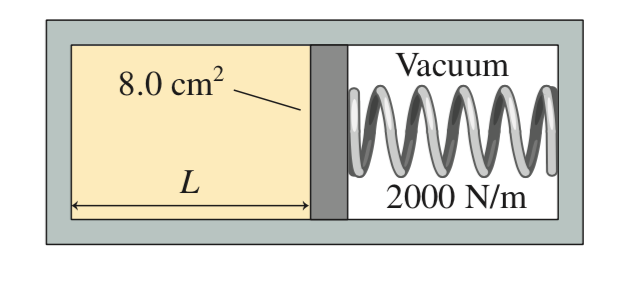
\includegraphics[width=0.5\linewidth]{Final_2}
\end{figure}

\section{RMS speed}
The rms speed of the molecules in 1.0g of hydrogen gas is 1800 m$/$s.
\begin{enumerate}
\item What is the total translational kinetic energy of the gas of molecules?
\item What is the thermal energy of the gas?
\item 500 J of work are done to compress the gas while, in the same process, 1200 J of heat energy are transferred from the gas to the environment. Afterward, what is the rms speed of the molecules?
\end{enumerate}

\section{Carnot heat engine and an ordinary fridge}
A Carnot heat engine and an ordinary refrigerator with coefficient of performance 2.00 operate between reservoirs at 350 K and 250 K. The work done by the Carnot heat engine drives the refrigerator. If the heat engine extracts 10.0 J of energy from the hot reservoir, how much energy does the refrigerator exhaust to the hot reservoir?

\section{Heat engine driving fridge}
The figure below shows a Carnot heat engine driving a Carnot refrigerator.

\begin{enumerate}
\item Determine $Q_1, Q_2, Q_3$.
\item Is $Q_3$ greater than, less than, or equal to $Q_1$?
\item Does this apparatus violate the second law of thermodynamics?

\begin{figure}[h!]
\centering
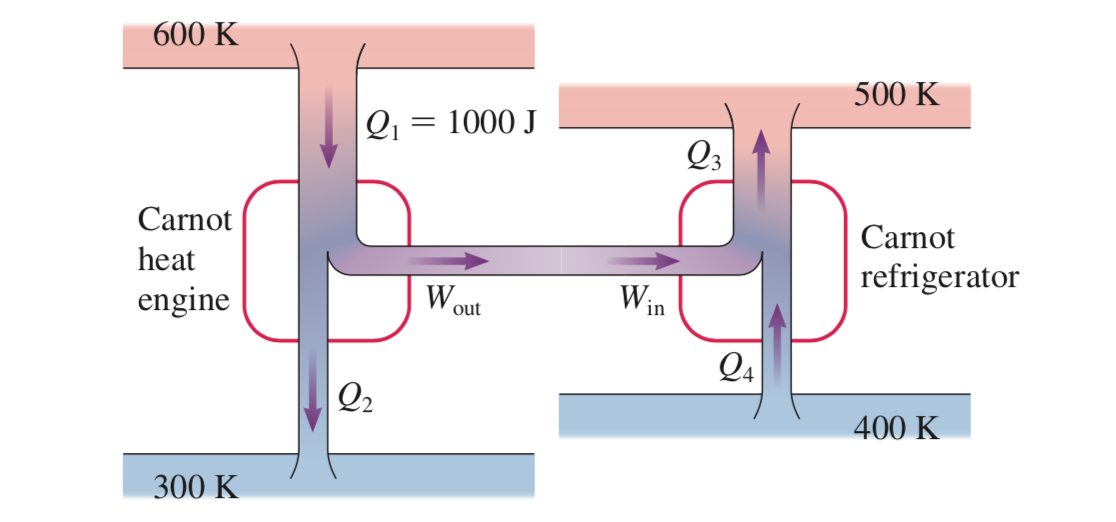
\includegraphics[width=0.5\linewidth]{Final_1}
\caption{Carnot heat engine driving Carnot fridge}
\end{figure}
\end{enumerate}



\end{document}
